% Options for packages loaded elsewhere
\PassOptionsToPackage{unicode}{hyperref}
\PassOptionsToPackage{hyphens}{url}
%
\documentclass[
]{article}
\title{Reproducible Research: Peer Assessment 1}
\author{}
\date{\vspace{-2.5em}}

\usepackage{amsmath,amssymb}
\usepackage{lmodern}
\usepackage{iftex}
\ifPDFTeX
  \usepackage[T1]{fontenc}
  \usepackage[utf8]{inputenc}
  \usepackage{textcomp} % provide euro and other symbols
\else % if luatex or xetex
  \usepackage{unicode-math}
  \defaultfontfeatures{Scale=MatchLowercase}
  \defaultfontfeatures[\rmfamily]{Ligatures=TeX,Scale=1}
\fi
% Use upquote if available, for straight quotes in verbatim environments
\IfFileExists{upquote.sty}{\usepackage{upquote}}{}
\IfFileExists{microtype.sty}{% use microtype if available
  \usepackage[]{microtype}
  \UseMicrotypeSet[protrusion]{basicmath} % disable protrusion for tt fonts
}{}
\makeatletter
\@ifundefined{KOMAClassName}{% if non-KOMA class
  \IfFileExists{parskip.sty}{%
    \usepackage{parskip}
  }{% else
    \setlength{\parindent}{0pt}
    \setlength{\parskip}{6pt plus 2pt minus 1pt}}
}{% if KOMA class
  \KOMAoptions{parskip=half}}
\makeatother
\usepackage{xcolor}
\IfFileExists{xurl.sty}{\usepackage{xurl}}{} % add URL line breaks if available
\IfFileExists{bookmark.sty}{\usepackage{bookmark}}{\usepackage{hyperref}}
\hypersetup{
  pdftitle={Reproducible Research: Peer Assessment 1},
  hidelinks,
  pdfcreator={LaTeX via pandoc}}
\urlstyle{same} % disable monospaced font for URLs
\usepackage[margin=1in]{geometry}
\usepackage{color}
\usepackage{fancyvrb}
\newcommand{\VerbBar}{|}
\newcommand{\VERB}{\Verb[commandchars=\\\{\}]}
\DefineVerbatimEnvironment{Highlighting}{Verbatim}{commandchars=\\\{\}}
% Add ',fontsize=\small' for more characters per line
\usepackage{framed}
\definecolor{shadecolor}{RGB}{248,248,248}
\newenvironment{Shaded}{\begin{snugshade}}{\end{snugshade}}
\newcommand{\AlertTok}[1]{\textcolor[rgb]{0.94,0.16,0.16}{#1}}
\newcommand{\AnnotationTok}[1]{\textcolor[rgb]{0.56,0.35,0.01}{\textbf{\textit{#1}}}}
\newcommand{\AttributeTok}[1]{\textcolor[rgb]{0.77,0.63,0.00}{#1}}
\newcommand{\BaseNTok}[1]{\textcolor[rgb]{0.00,0.00,0.81}{#1}}
\newcommand{\BuiltInTok}[1]{#1}
\newcommand{\CharTok}[1]{\textcolor[rgb]{0.31,0.60,0.02}{#1}}
\newcommand{\CommentTok}[1]{\textcolor[rgb]{0.56,0.35,0.01}{\textit{#1}}}
\newcommand{\CommentVarTok}[1]{\textcolor[rgb]{0.56,0.35,0.01}{\textbf{\textit{#1}}}}
\newcommand{\ConstantTok}[1]{\textcolor[rgb]{0.00,0.00,0.00}{#1}}
\newcommand{\ControlFlowTok}[1]{\textcolor[rgb]{0.13,0.29,0.53}{\textbf{#1}}}
\newcommand{\DataTypeTok}[1]{\textcolor[rgb]{0.13,0.29,0.53}{#1}}
\newcommand{\DecValTok}[1]{\textcolor[rgb]{0.00,0.00,0.81}{#1}}
\newcommand{\DocumentationTok}[1]{\textcolor[rgb]{0.56,0.35,0.01}{\textbf{\textit{#1}}}}
\newcommand{\ErrorTok}[1]{\textcolor[rgb]{0.64,0.00,0.00}{\textbf{#1}}}
\newcommand{\ExtensionTok}[1]{#1}
\newcommand{\FloatTok}[1]{\textcolor[rgb]{0.00,0.00,0.81}{#1}}
\newcommand{\FunctionTok}[1]{\textcolor[rgb]{0.00,0.00,0.00}{#1}}
\newcommand{\ImportTok}[1]{#1}
\newcommand{\InformationTok}[1]{\textcolor[rgb]{0.56,0.35,0.01}{\textbf{\textit{#1}}}}
\newcommand{\KeywordTok}[1]{\textcolor[rgb]{0.13,0.29,0.53}{\textbf{#1}}}
\newcommand{\NormalTok}[1]{#1}
\newcommand{\OperatorTok}[1]{\textcolor[rgb]{0.81,0.36,0.00}{\textbf{#1}}}
\newcommand{\OtherTok}[1]{\textcolor[rgb]{0.56,0.35,0.01}{#1}}
\newcommand{\PreprocessorTok}[1]{\textcolor[rgb]{0.56,0.35,0.01}{\textit{#1}}}
\newcommand{\RegionMarkerTok}[1]{#1}
\newcommand{\SpecialCharTok}[1]{\textcolor[rgb]{0.00,0.00,0.00}{#1}}
\newcommand{\SpecialStringTok}[1]{\textcolor[rgb]{0.31,0.60,0.02}{#1}}
\newcommand{\StringTok}[1]{\textcolor[rgb]{0.31,0.60,0.02}{#1}}
\newcommand{\VariableTok}[1]{\textcolor[rgb]{0.00,0.00,0.00}{#1}}
\newcommand{\VerbatimStringTok}[1]{\textcolor[rgb]{0.31,0.60,0.02}{#1}}
\newcommand{\WarningTok}[1]{\textcolor[rgb]{0.56,0.35,0.01}{\textbf{\textit{#1}}}}
\usepackage{graphicx}
\makeatletter
\def\maxwidth{\ifdim\Gin@nat@width>\linewidth\linewidth\else\Gin@nat@width\fi}
\def\maxheight{\ifdim\Gin@nat@height>\textheight\textheight\else\Gin@nat@height\fi}
\makeatother
% Scale images if necessary, so that they will not overflow the page
% margins by default, and it is still possible to overwrite the defaults
% using explicit options in \includegraphics[width, height, ...]{}
\setkeys{Gin}{width=\maxwidth,height=\maxheight,keepaspectratio}
% Set default figure placement to htbp
\makeatletter
\def\fps@figure{htbp}
\makeatother
\setlength{\emergencystretch}{3em} % prevent overfull lines
\providecommand{\tightlist}{%
  \setlength{\itemsep}{0pt}\setlength{\parskip}{0pt}}
\setcounter{secnumdepth}{-\maxdimen} % remove section numbering
\ifLuaTeX
  \usepackage{selnolig}  % disable illegal ligatures
\fi

\begin{document}
\maketitle

\hypertarget{loading-and-preprocessing-the-data}{%
\subsection{Loading and preprocessing the
data}\label{loading-and-preprocessing-the-data}}

\begin{Shaded}
\begin{Highlighting}[]
\NormalTok{activity }\OtherTok{\textless{}{-}} \FunctionTok{read.csv}\NormalTok{(}\StringTok{"activity.csv"}\NormalTok{)}
\end{Highlighting}
\end{Shaded}

\hypertarget{what-is-mean-total-number-of-steps-taken-per-day}{%
\subsection{What is mean total number of steps taken per
day?}\label{what-is-mean-total-number-of-steps-taken-per-day}}

\begin{Shaded}
\begin{Highlighting}[]
\FunctionTok{library}\NormalTok{(dplyr)}

\NormalTok{totalSteps }\OtherTok{\textless{}{-}}\NormalTok{ activity }\SpecialCharTok{\%\textgreater{}\%} \FunctionTok{select}\NormalTok{(steps, date) }\SpecialCharTok{\%\textgreater{}\%}
     \FunctionTok{group\_by}\NormalTok{(date) }\SpecialCharTok{\%\textgreater{}\%}
     \FunctionTok{summarise}\NormalTok{(}\AttributeTok{total\_steps =} \FunctionTok{sum}\NormalTok{(steps, }\AttributeTok{na.rm =} \ConstantTok{TRUE}\NormalTok{))}

\FunctionTok{hist}\NormalTok{(totalSteps}\SpecialCharTok{$}\NormalTok{total\_steps, }\AttributeTok{xlab =} \StringTok{"Total Steps Per Day"}\NormalTok{, }\AttributeTok{main =} \StringTok{"Histogram of Steps Per Day"}\NormalTok{)}
\end{Highlighting}
\end{Shaded}

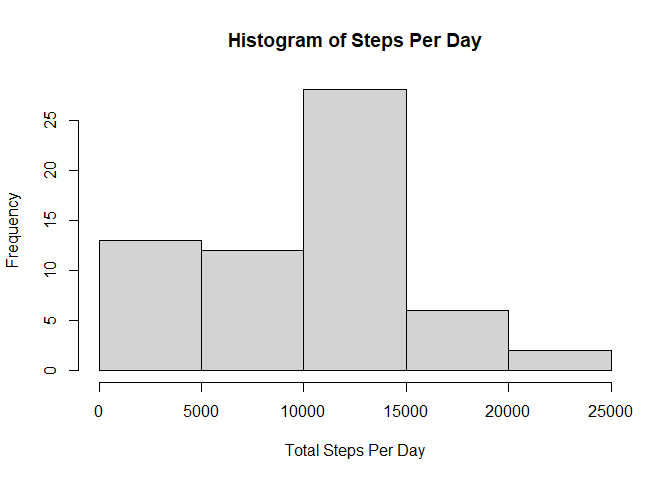
\includegraphics{PA1_template_files/figure-latex/unnamed-chunk-2-1.pdf}

\hypertarget{mean-and-median-values}{%
\subsubsection{Mean and Median values}\label{mean-and-median-values}}

\hypertarget{mean}{%
\paragraph{Mean}\label{mean}}

\begin{Shaded}
\begin{Highlighting}[]
\FunctionTok{mean}\NormalTok{(totalSteps}\SpecialCharTok{$}\NormalTok{total\_steps)}
\end{Highlighting}
\end{Shaded}

\begin{verbatim}
## [1] 9354.23
\end{verbatim}

\hypertarget{median}{%
\paragraph{Median}\label{median}}

\begin{Shaded}
\begin{Highlighting}[]
\FunctionTok{median}\NormalTok{(totalSteps}\SpecialCharTok{$}\NormalTok{total\_steps)}
\end{Highlighting}
\end{Shaded}

\begin{verbatim}
## [1] 10395
\end{verbatim}

\hypertarget{what-is-the-average-daily-activity-pattern}{%
\subsection{What is the average daily activity
pattern?}\label{what-is-the-average-daily-activity-pattern}}

\begin{Shaded}
\begin{Highlighting}[]
\NormalTok{averageStespsDF }\OtherTok{\textless{}{-}}\NormalTok{ activity }\SpecialCharTok{\%\textgreater{}\%} \FunctionTok{select}\NormalTok{(steps, interval) }\SpecialCharTok{\%\textgreater{}\%}
     \FunctionTok{group\_by}\NormalTok{(interval) }\SpecialCharTok{\%\textgreater{}\%}
     \FunctionTok{summarise}\NormalTok{(}\AttributeTok{average\_steps =} \FunctionTok{mean}\NormalTok{(steps, }\AttributeTok{na.rm =} \ConstantTok{TRUE}\NormalTok{))}

\FunctionTok{plot}\NormalTok{(averageStespsDF}\SpecialCharTok{$}\NormalTok{interval, averageStespsDF}\SpecialCharTok{$}\NormalTok{average\_steps, }\AttributeTok{type =} \StringTok{"l"}\NormalTok{, }\AttributeTok{xlab =} \StringTok{"Time Interval"}\NormalTok{, }\AttributeTok{ylab =} \StringTok{"Average Steps"}\NormalTok{)}
\end{Highlighting}
\end{Shaded}

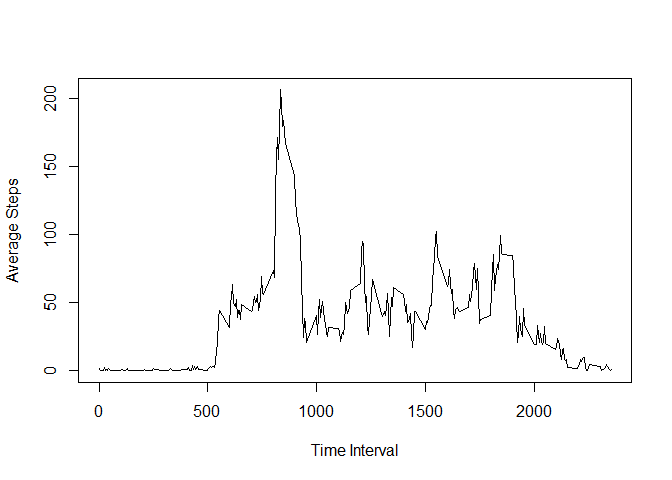
\includegraphics{PA1_template_files/figure-latex/unnamed-chunk-5-1.pdf}

\begin{Shaded}
\begin{Highlighting}[]
\NormalTok{maxStepsInterval }\OtherTok{\textless{}{-}}\NormalTok{ averageStespsDF }\SpecialCharTok{\%\textgreater{}\%} \FunctionTok{filter}\NormalTok{(average\_steps }\SpecialCharTok{==} \FunctionTok{max}\NormalTok{(average\_steps))}
\end{Highlighting}
\end{Shaded}

\hypertarget{max-steps-interval}{%
\paragraph{Max Steps Interval}\label{max-steps-interval}}

\begin{Shaded}
\begin{Highlighting}[]
\NormalTok{maxStepsInterval}\SpecialCharTok{$}\NormalTok{interval[}\DecValTok{1}\NormalTok{]}
\end{Highlighting}
\end{Shaded}

\begin{verbatim}
## [1] 835
\end{verbatim}

\hypertarget{imputing-missing-values}{%
\subsection{Imputing missing values}\label{imputing-missing-values}}

\hypertarget{number-of-missing-values}{%
\paragraph{Number of Missing Values}\label{number-of-missing-values}}

\begin{Shaded}
\begin{Highlighting}[]
\NormalTok{nas }\OtherTok{\textless{}{-}}\NormalTok{ activity }\SpecialCharTok{\%\textgreater{}\%} \FunctionTok{filter}\NormalTok{(}\FunctionTok{is.na}\NormalTok{(interval) }\SpecialCharTok{|} \FunctionTok{is.na}\NormalTok{(steps))}
\CommentTok{\#number of missing values}
\FunctionTok{dim}\NormalTok{(nas)[}\DecValTok{1}\NormalTok{]}
\end{Highlighting}
\end{Shaded}

\begin{verbatim}
## [1] 2304
\end{verbatim}

\begin{Shaded}
\begin{Highlighting}[]
\NormalTok{imputedDf }\OtherTok{\textless{}{-}}\NormalTok{ activity}
\NormalTok{con }\OtherTok{\textless{}{-}} \FunctionTok{is.na}\NormalTok{(activity}\SpecialCharTok{$}\NormalTok{steps)}
\NormalTok{imputedDf[con,]}\SpecialCharTok{$}\NormalTok{steps }\OtherTok{\textless{}{-}} \FunctionTok{mean}\NormalTok{(imputedDf}\SpecialCharTok{$}\NormalTok{steps, }\AttributeTok{na.rm =} \ConstantTok{TRUE}\NormalTok{)}


\NormalTok{imputedTotalSteps }\OtherTok{\textless{}{-}}\NormalTok{ imputedDf }\SpecialCharTok{\%\textgreater{}\%} \FunctionTok{select}\NormalTok{(steps, date) }\SpecialCharTok{\%\textgreater{}\%}
     \FunctionTok{group\_by}\NormalTok{(date) }\SpecialCharTok{\%\textgreater{}\%}
     \FunctionTok{summarise}\NormalTok{(}\AttributeTok{total\_steps =} \FunctionTok{sum}\NormalTok{(steps))}

\FunctionTok{hist}\NormalTok{(imputedTotalSteps}\SpecialCharTok{$}\NormalTok{total\_steps, }\AttributeTok{xlab =} \StringTok{"Total Steps"}\NormalTok{, }\AttributeTok{main =} \StringTok{"Histogram of Total Steps"}\NormalTok{)}
\end{Highlighting}
\end{Shaded}

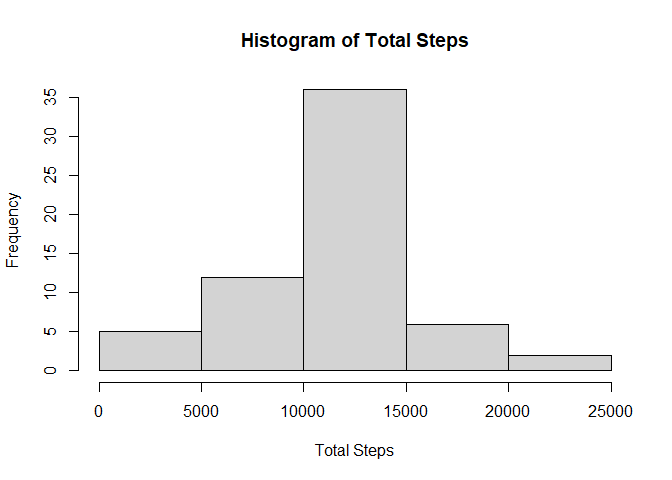
\includegraphics{PA1_template_files/figure-latex/unnamed-chunk-8-1.pdf}

\hypertarget{mean-value}{%
\paragraph{Mean Value}\label{mean-value}}

\begin{Shaded}
\begin{Highlighting}[]
\FunctionTok{mean}\NormalTok{(imputedTotalSteps}\SpecialCharTok{$}\NormalTok{total\_steps)}
\end{Highlighting}
\end{Shaded}

\begin{verbatim}
## [1] 10766.19
\end{verbatim}

\hypertarget{median-value}{%
\paragraph{Median Value}\label{median-value}}

\begin{Shaded}
\begin{Highlighting}[]
\FunctionTok{median}\NormalTok{(imputedTotalSteps}\SpecialCharTok{$}\NormalTok{total\_steps)}
\end{Highlighting}
\end{Shaded}

\begin{verbatim}
## [1] 10766.19
\end{verbatim}

\hypertarget{impact-of-imputing-data}{%
\paragraph{Impact of Imputing Data}\label{impact-of-imputing-data}}

\hypertarget{we-can-see-that-imputing-data-has-changed-the-values-of-mean-and-median-because-we-changed-the-data-also-it-made-the-mean-very-close-to-the-mediane-because-more-values-are-now-equals-the-mean-so-its-more-likely-that-the-middle-value-will-be-the-mean.}{%
\subparagraph{We can see that imputing Data has changed The values of
mean and median because we changed the data, also it made the mean very
close to the mediane because more values are now equals the mean So it's
more likely that the middle value will be the
mean.}\label{we-can-see-that-imputing-data-has-changed-the-values-of-mean-and-median-because-we-changed-the-data-also-it-made-the-mean-very-close-to-the-mediane-because-more-values-are-now-equals-the-mean-so-its-more-likely-that-the-middle-value-will-be-the-mean.}}

\hypertarget{are-there-differences-in-activity-patterns-between-weekdays-and-weekends}{%
\subsection{Are there differences in activity patterns between weekdays
and
weekends?}\label{are-there-differences-in-activity-patterns-between-weekdays-and-weekends}}

\begin{Shaded}
\begin{Highlighting}[]
\FunctionTok{library}\NormalTok{(lattice)}

\NormalTok{weekDays }\OtherTok{\textless{}{-}}\NormalTok{ imputedDf }\SpecialCharTok{\%\textgreater{}\%} \FunctionTok{mutate}\NormalTok{(}\AttributeTok{weekDay =} \FunctionTok{weekdays}\NormalTok{(}\FunctionTok{as.POSIXlt}\NormalTok{(date)), }\AttributeTok{fweekDay =} \StringTok{"f"}\NormalTok{)}


\NormalTok{weekDays[weekDays}\SpecialCharTok{$}\NormalTok{weekDay }\SpecialCharTok{\%in\%} \FunctionTok{c}\NormalTok{(}\StringTok{"Saturday"}\NormalTok{, }\StringTok{"Sunday"}\NormalTok{),]}\SpecialCharTok{$}\NormalTok{fweekDay }\OtherTok{\textless{}{-}} \StringTok{"weekend"}
\NormalTok{weekDays[}\SpecialCharTok{!}\NormalTok{( weekDays}\SpecialCharTok{$}\NormalTok{weekDay }\SpecialCharTok{\%in\%} \FunctionTok{c}\NormalTok{(}\StringTok{"Saturday"}\NormalTok{, }\StringTok{"Sunday"}\NormalTok{)),]}\SpecialCharTok{$}\NormalTok{fweekDay }\OtherTok{\textless{}{-}} \StringTok{"weekday"}

\NormalTok{weekDays }\OtherTok{\textless{}{-}}\NormalTok{ weekDays }\SpecialCharTok{\%\textgreater{}\%} \FunctionTok{mutate}\NormalTok{(}\AttributeTok{weekDay =} \FunctionTok{as.factor}\NormalTok{(weekDay))}

\NormalTok{weekDays }\OtherTok{\textless{}{-}}\NormalTok{ weekDays }\SpecialCharTok{\%\textgreater{}\%}
     \FunctionTok{group\_by}\NormalTok{(interval, fweekDay) }\SpecialCharTok{\%\textgreater{}\%}
     \FunctionTok{summarise}\NormalTok{(}\AttributeTok{average\_steps =} \FunctionTok{mean}\NormalTok{(steps))}

\FunctionTok{xyplot}\NormalTok{(average\_steps}\SpecialCharTok{\textasciitilde{}}\NormalTok{interval}\SpecialCharTok{|}\NormalTok{fweekDay, }\AttributeTok{type =} \StringTok{"l"}\NormalTok{, }\AttributeTok{data =}\NormalTok{ weekDays, }\AttributeTok{groups =}\NormalTok{ fweekDay, }\AttributeTok{layout =} \FunctionTok{c}\NormalTok{(}\DecValTok{2}\NormalTok{, }\DecValTok{1}\NormalTok{), }\AttributeTok{ylab =} \StringTok{"Average Steps."}\NormalTok{)}
\end{Highlighting}
\end{Shaded}

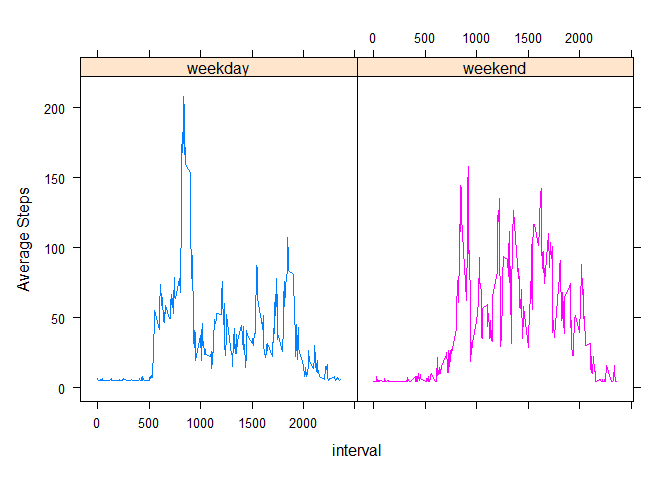
\includegraphics{PA1_template_files/figure-latex/unnamed-chunk-11-1.pdf}

\end{document}
